\documentclass{report} % Add the document class
\usepackage{graphicx} % For including graphics like logos
\usepackage{lipsum}   % For dummy text
\usepackage{setspace} % For line spacing
\usepackage{fancyhdr} % For custom headers and footers
\usepackage{geometry} % For page margins
\usepackage{amsmath} % For mathematical equations
\usepackage{enumitem} % For customized lists
\usepackage{amsfonts} % For the \forall symbol
\usepackage{multicol} % For multiple columns if needed
\usepackage{amsmath} % For additional math formatting
\usepackage{enumitem} % For customizing lists
\usepackage{acronym} % For defining acronyms
\usepackage{hyperref} % For hyperlinks for table of contents
\usepackage{tocbibind} % For adding list of figures, tables to table of contents
\geometry{top=1in, bottom=1in, left=1in, right=1in} % Set page margins

% Configure the hyperref package to remove red boxes and customize link colors
\hypersetup{
    colorlinks=true,      % Set to true to enable colored links
    linkcolor=black,       % Color for internal links (sections, pages, etc.)
    citecolor=black,       % Color for citation links
    filecolor=black,       % Color for file links
    urlcolor=black         % Color for URL links
}

\begin{document}

% Set up the header and footer using fancyhdr
% \pagestyle{fancy}
% \fancyhf{} % Clear all header and footer fields

% % Define the header
% \fancyhead[L]{
%     \small
%     Technical University of Applied Sciences Würzburg-Schweinfurt (THWS)\\
%     Faculty of Computer Science and Business Information Systems
% }

% % Adjust the header position
% \renewcommand{\headrulewidth}{0pt} % Remove the header rule line


% Title Page
\begin{titlepage}
    \centering
    \vspace*{1cm}
    
    \Large \textbf{Technical University of Applied Sciences Würzburg-Schweinfurt (THWS)}\\
    \vspace{0.5cm}
    \Large Faculty of Computer Science and Business Information Systems\\
    \vspace{1cm}
    
    \huge \textbf{Master Thesis}\\
    \vspace{1.5cm}
    
    \Huge \textbf{Electric Motor Modelling via Graph Neural Networks}\\
    \vspace{2cm}
    
    \large \textbf{Submitted to the Technical University of Applied Sciences Würzburg-Schweinfurt in the Faculty of Computer Science and Business Information Systems to
    complete a course of studies in Master of Artificial Intelligence}
    
    \vspace{1cm}
    
    \huge Lilly Abraham\\
    \huge K64889\\
    \vspace{1cm}
    \large To be Submitted on: 11.12.2024\\ % replace with Submitted on
    
    \vfill
    
    \large
    Initial examiner: Prof. Dr. Magda Gregorova\\
    Secondary examiner: Prof. Gracia Herranz Mercedes\\

\end{titlepage}

\newpage % Start a new page


% Including an image on this page
\begin{figure}[h]
    
\includegraphics[width=0.8\textwidth]{./ReportImages/qrcode.png} % Adjust path and filename
    \label{fig:your-image}
\end{figure}

\newpage % Start a new page

\chapter*{Abstract}
\addcontentsline{toc}{chapter}{Abstract}

The thesis explores an approach to predict KPIs of topology invariant IPSM Electric Motors by transforming its geometric, physical and simulation parameters into a graph representation. \\
The KPIs to be predicted are plots on Efficiency grid(3D) and Torque curve(2D).\\
We aim to first parameterize the EM design such that it is feasible to convert into a graph representation. \\
Next, we would create a Graph with relevant attributes and design a GNN with the graph as input and the plots in the format of vectors as target values.\\
Additionally we may also need to customize the loss function in a way that would smoothen out the plot curves of the prediction values.\\
Then, we would evaluate the predictions with the test target values by experimenting with various hyperparameter tuning settings and as a baseline with an MLP model of the parameters in tabular form.\\
Finally we will enable the KPI's plot visualisation in a manner presentable to the client Valeo(Automaker Company).\\

\section*{Abstrakt}
The aim of the Master Thesis is to train a neural network to learn the parameters of Electric Motors and thus be able to predict its KPIs.
The KPIs are 2D and 3D plots on Torque(Mgrenz) curve(Mgrenz) and Efficiency grid(ETA). Other KPIs can be calculated from these two KPIs.
For instance the Vibration Costs are inversely proportional to the Efficieny values predicted. 


\newpage 

\newpage 

\chapter*{Acknowledgement}
\addcontentsline{toc}{chapter}{Acknowledgement}
I would like to thank my supervisor Prof. Dr. Magda Gregorova for her guidance and support throughout the course of this thesis and Valeo for providing the data.
Special thanks to Mr Daniel and Leo for sharing valuable insights of the data from a electromechanincal standpoint.

\newpage

\newpage

\begin{spacing}{1.2}
    \tableofcontents
\end{spacing}

\newpage

\newpage

\chapter*{Abbreviations}
\addcontentsline{toc}{chapter}{Abbreviations}
\begin{acronym}[TDMA]
  
    \acro{GNN :}{Graph Neural Network}
    \acro{MLP :}{Multi Linear Perceptron}
    \acro{GNN :}{Graph Neural Network}
    \acro{KPI :}{Key Performance Indicator}
    \acro{EM :}{Electric Motor}
    \acro{FEM :}{Finite Element Method}
    \acro{CNN :}{Convolution Neural Network}
    \acro{2D :}{2 Dimension}
    \acro{3D :}{3 Dimension}

\end{acronym}

\newpage

\newpage

\chapter*{Introduction} 
\addcontentsline{toc}{chapter}{Introduction}
In the design of electric motors vast amounts of data are generated to determine which design of an EM fits best to KPIs. \\
KPIs of an Electric Motor are essential to judge the performance of the motor before it is manufactured. \\
Traditionally these KPIs are inferred from a description of an EM design via a FEM approximating the solutions of the Maxwell’s equations. This process, though well established in the EM design, is very time consuming and does not allow for high-throughput engine design optimization. \\
The actual engine data of Valeo is used here as the dataset comprising of multiple variant designs of the Double-V topology.\\
The 3 motor topologies manufactured by Valeo are as below:


% \begin{figure}[h]
%     \centering
%     \begin{minipage}[b]{0.3\textwidth}
%         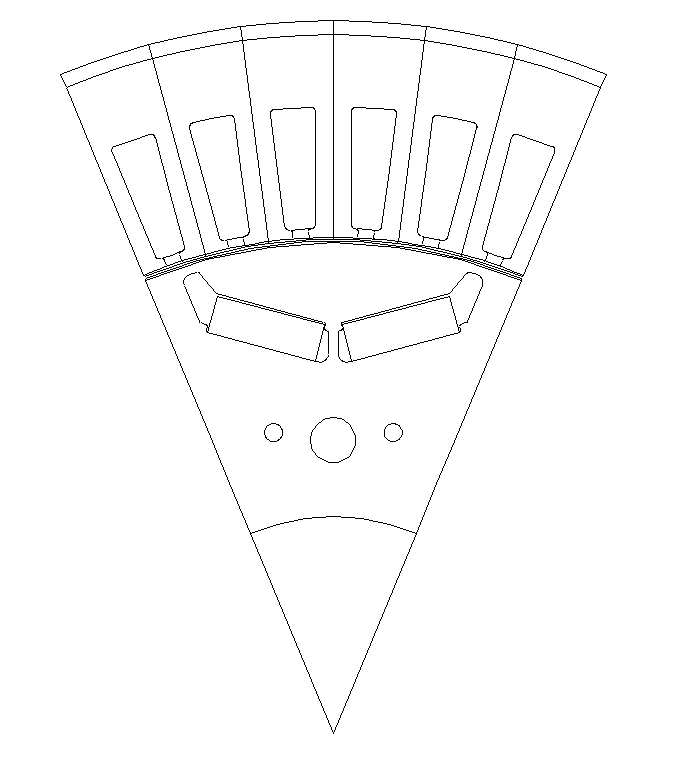
\includegraphics[width=\textwidth]{./ReportImages/1V_Magnet.png}
%         \caption{V1 Magnet(Source:Valeo)}
%         \label{fig:V1 Magnet}
%     \end{minipage}
%     \hfill
%     \begin{minipage}[b]{0.3\textwidth}
%         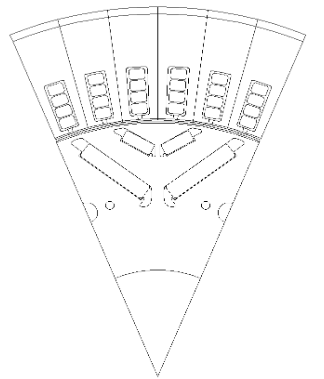
\includegraphics[width=\textwidth]{./ReportImages/2V_Magnet.png}
%         \caption{V2 Magnet(Source:Valeo)}
%         \label{fig:V2 Magnet}
%     \end{minipage}
%     \hfill
%     \begin{minipage}[b]{0.3\textwidth}
%         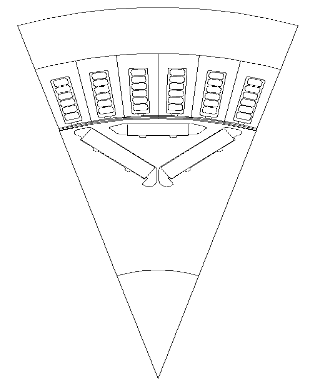
\includegraphics[width=\textwidth]{./ReportImages/Nabla_Magnet.png}
%         \caption{Nabla Magnet(Source:Valeo)}
%         \label{fig:Nabla Magnet}
%     \end{minipage}
% \end{figure}

\begin{figure}[h]
    \centering
    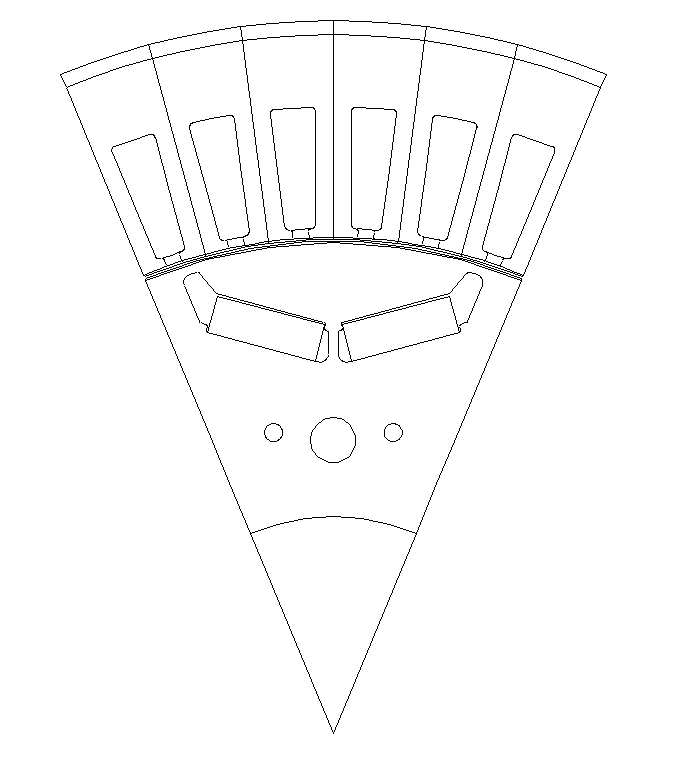
\includegraphics[width=0.25\textwidth]{./ReportImages/1V_Magnet.png}
    \caption{V1 Magnet(Source:Valeo)}
    \label{fig:V1 Magnet}
\end{figure}

\begin{figure}[h]
    \centering
    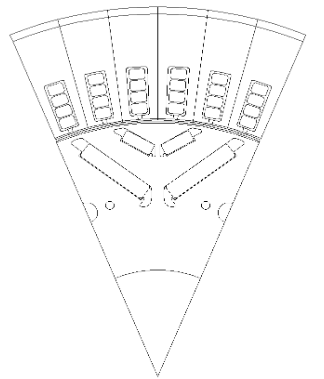
\includegraphics[width=0.25\textwidth]{./ReportImages/2V_Magnet.png}
    \caption{V2 Magnet(Source:Valeo)}
    \label{fig:V2 Magnet}
\end{figure}

\begin{figure}[h]
    \centering
    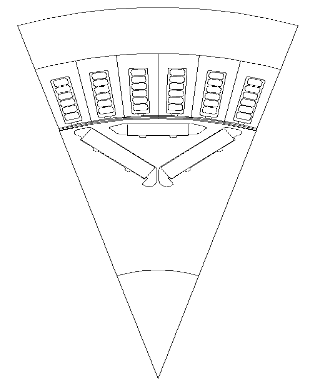
\includegraphics[width=0.25\textwidth]{./ReportImages/Nabla_Magnet.png}
    \caption{Nabla Magnet(Source:Valeo)}
    \label{fig:Nabla Magnet}
\end{figure}

This master thesis explores a way to do surrogate modelling of the current process as is highlighted in Figure \ref{fig:EM Design Flowchart} by making use of GNN/MLP for the modelling of electrical engine designs described parameterically. \\
\begin{figure}[h]
    \centering
    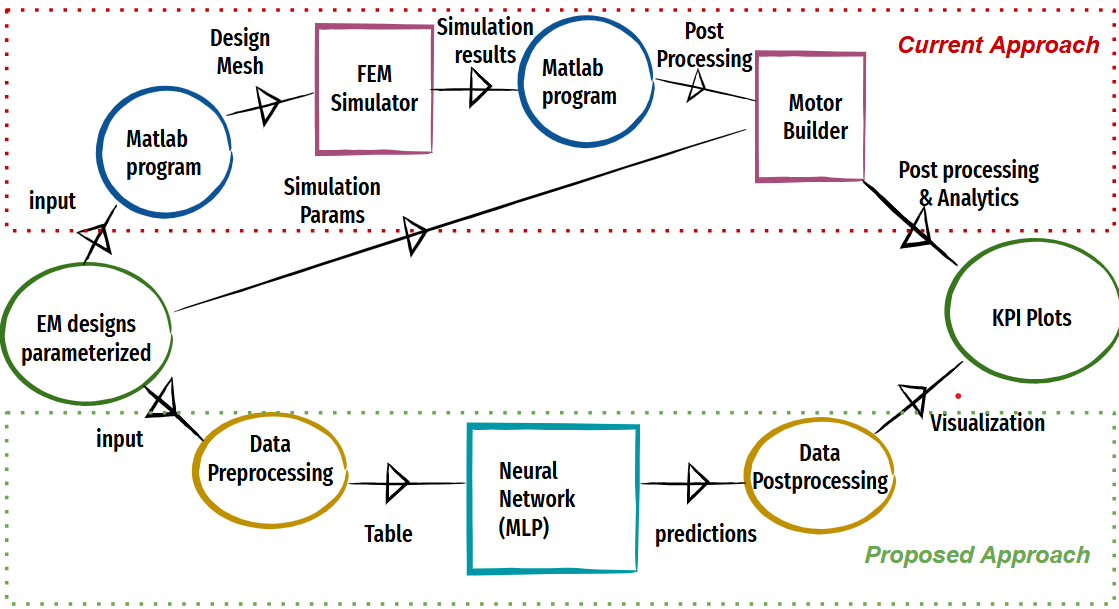
\includegraphics[width=0.9\textwidth]{./ReportImages/EM_design_flowchart_v2.png} 
    \caption{EM Design Flowchart}
    \label{fig:EM Design Flowchart}
\end{figure}

The thesis is structured to follow sections namely Literature Review, Dataset, Modelling, Experiments and Results, Conclusion, Appendix and Bibliography.\\
The Literature Review section will cover the related works that has been done in this domain. In the Dataset section a detailed insight to how our data is structured is given.
In the Modelling section, the methodologies used to tackle the problem will be further elaborated on. The Experiments and Results chapter will give insight on the outcomes of our work in addition to other findings we unearth. 
Conclusion chapter would summarize the entire thesis briefly and would also give a small glimpse into areas of improvement. Finally the Bibliography section lists out the articles cited for this thesis.\\
\newpage 

\chapter*{Literature Review} 
\addcontentsline{toc}{chapter}{Literature Review}
There has been extensive research in modeling the Electric Motor with CNN based on the images of the motor cross-section. 
However our approach is progressive in the sense that once the KPIs are predicted we would like to be able to generate the inputs and generating images is not ideal for our usecase.
Instead by generating the parameters of the motor we can be rest assured of more precise results. Hence the need to focus on the inputs as they are with their parametric description.
Literature also covers works on modelling this work as tabular data using MLPs. Although this is fairly good forseeing the impact of generating the inverse process yet MLPs cannot necessarily learn all the intricacies within motor components.
Hence the need to better represent the data typically in the form of graphs and model Graph Neural Networks to achieve the desired results. There has been close to no work of GNNs in this domain.
Although we see progress of GNNs in molecular chemistry, social networks usecases from which we draw inspiration from.

\newpage 

\chapter*{Dataset} 
\addcontentsline{toc}{chapter}{Dataset}
Valeo an automotive company has supplied the dataset consisting of close to 1500 Double V Electric Motor parameters. 
There are close to 196 parameters which comprises of the geometric, physical and simulation properties of the motor.

The geometry of a whole Double V motor is as below

\begin{figure}[h]
    \centering
    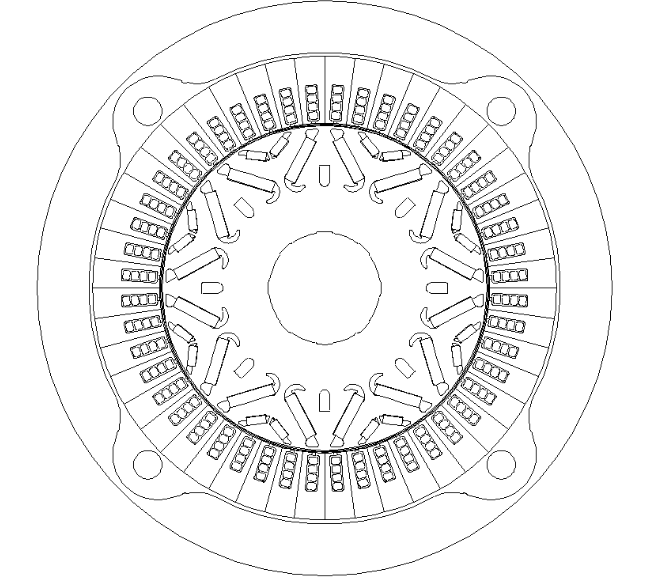
\includegraphics[width=0.5\textwidth]{./ReportImages/FullMotorv2.png} 
    \caption{Complete EM Geometry(Source:Valeo)}
    \label{fig:Full Motor}
\end{figure}

Below is the geometry of 1/8 cross-section of the same motor.

\begin{figure}[h]
    \centering
    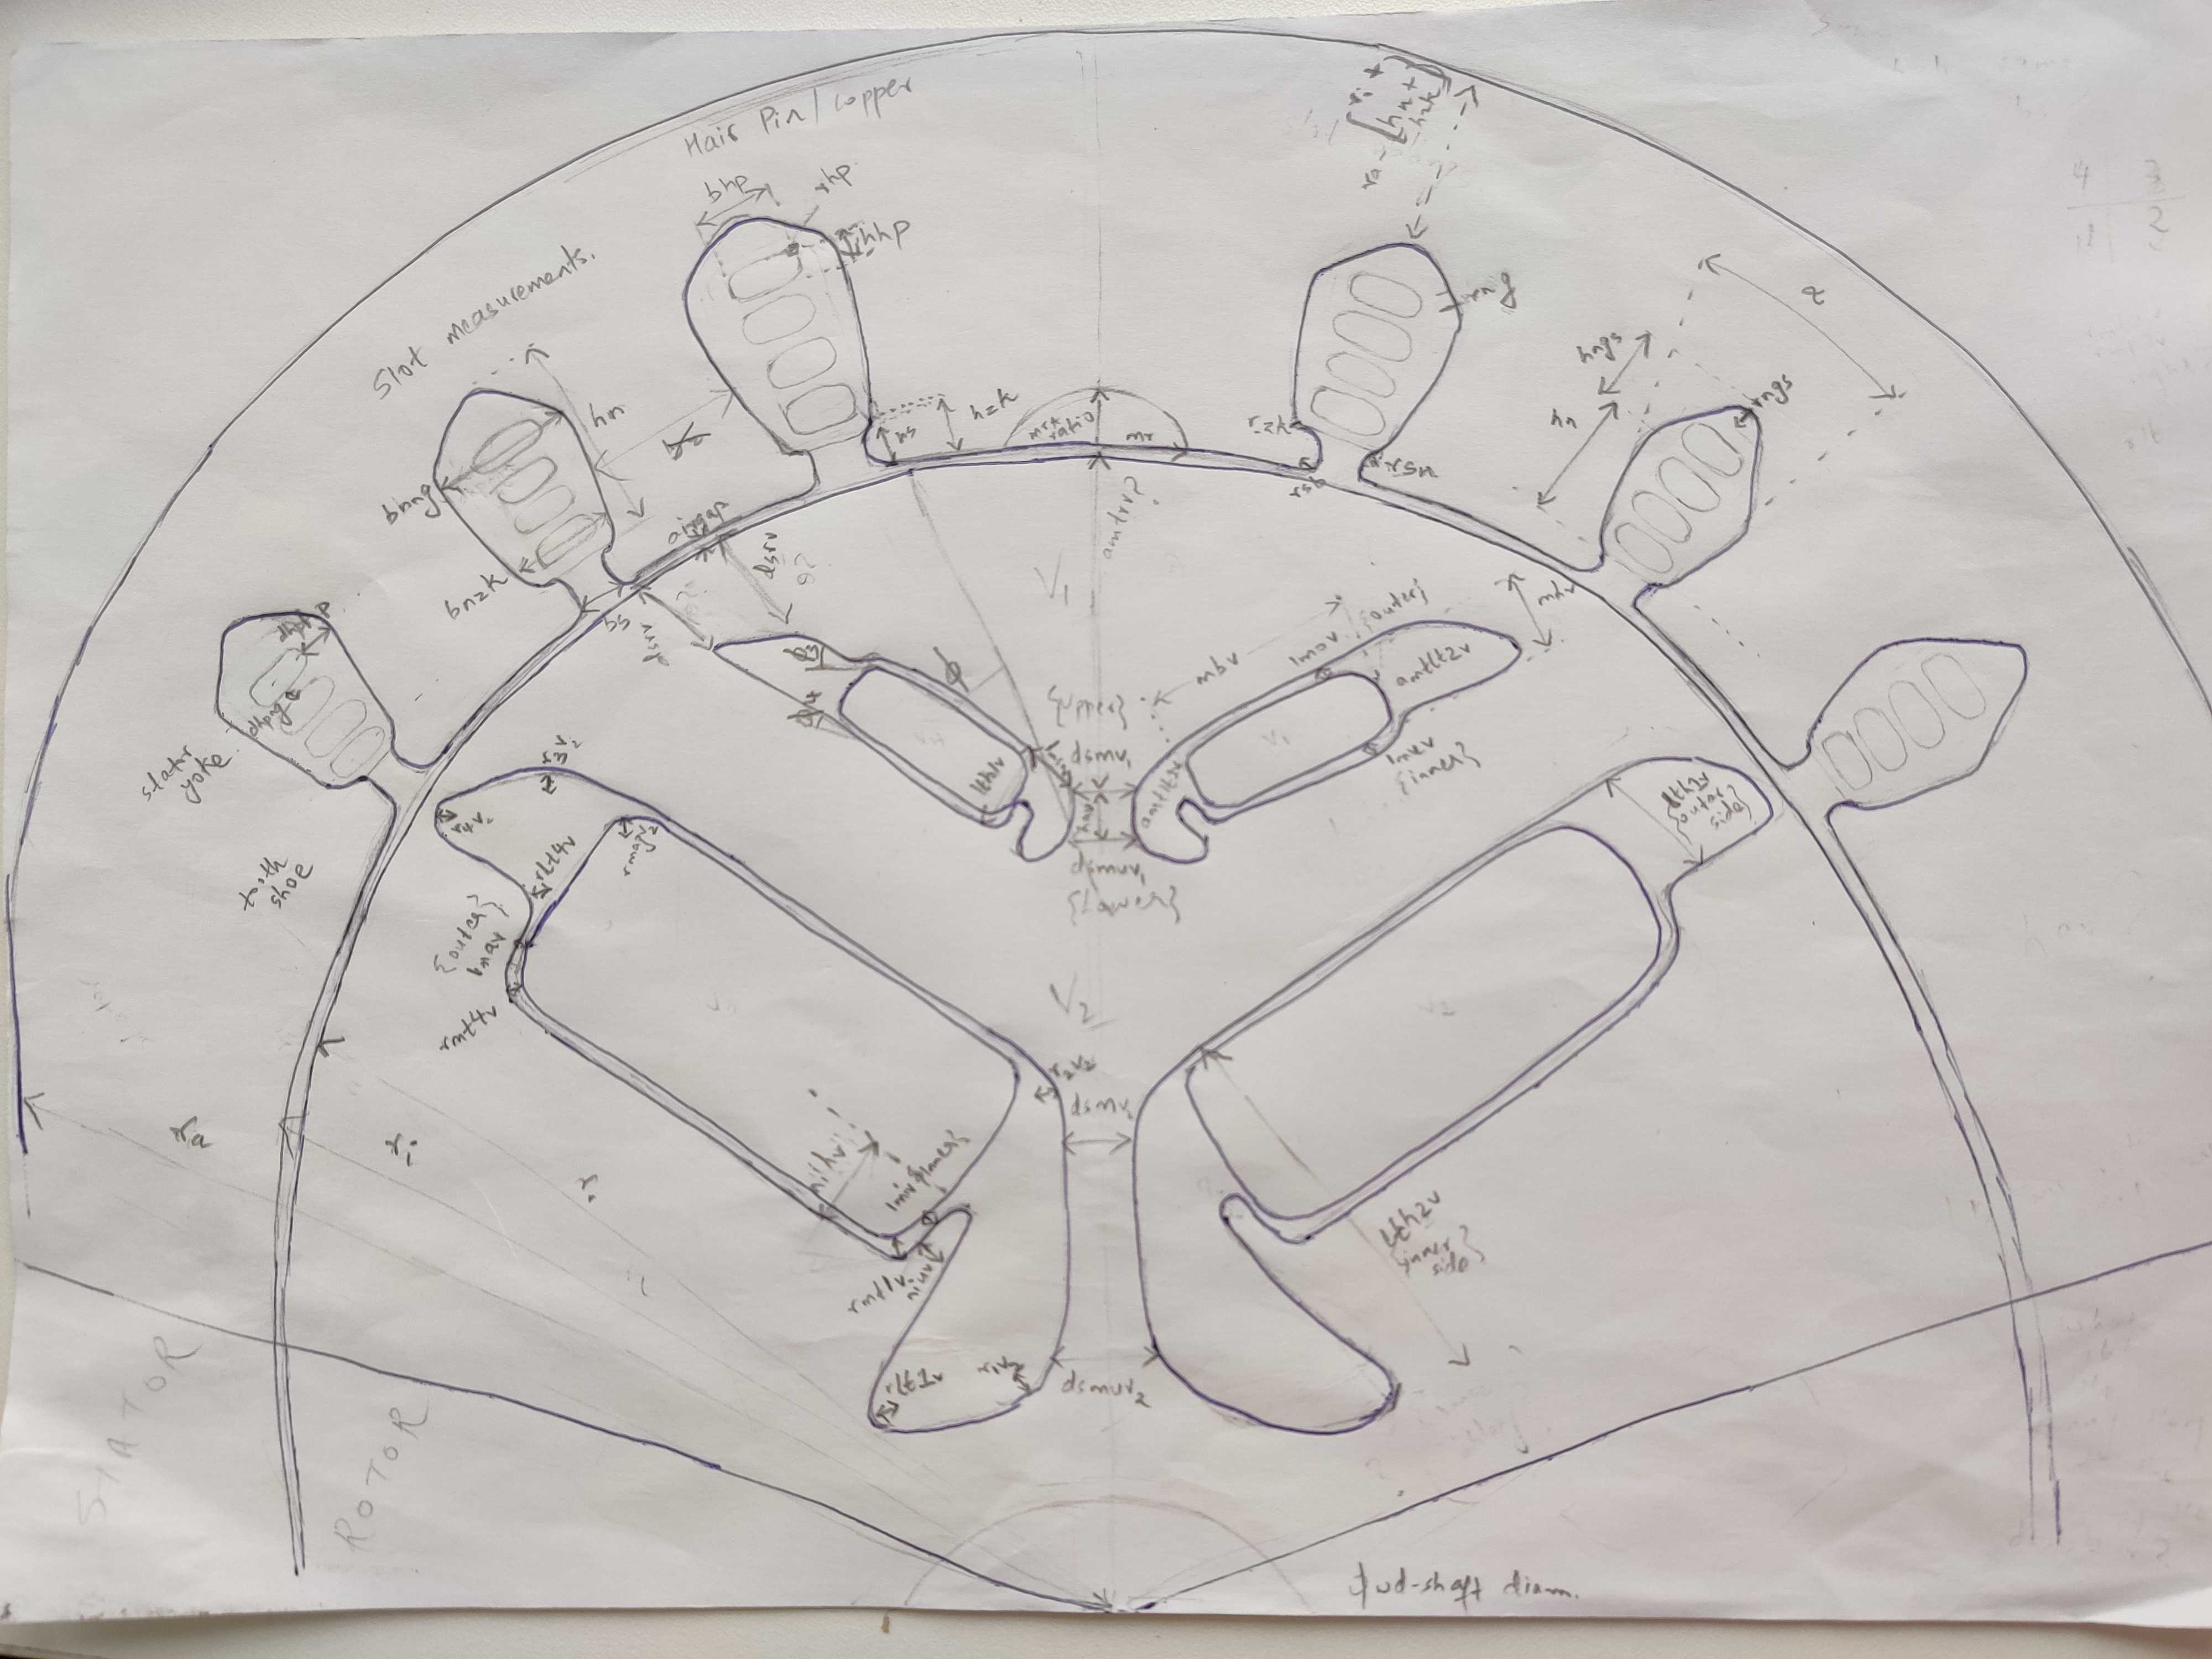
\includegraphics[width=0.5\textwidth]{./ReportImages/EMCrosssection.jpg} 
    \caption{1/8 Motor Crossection}
    \label{fig:1/8 Motor Crossection}
\end{figure}

\newpage 

For modelling the GNN, we represent the data in the form of a heterogeneous graph with different node and edge types.\\



\textbf{Node types}

\begin{enumerate}
    \item \textbf{General}
    
    \begin{itemize}
        \item General parameters:
        \[
            r = \{r_{i}\} \quad \forall i \in \{a, r, o\} 
        \]
        
        \textit{where:
        \begin{itemize}
            \item $r_{a}$: Outer Radius of the Stator
            \item $r_{r}$: Outer Radius of the Rotor
            \item $r_{o}$: Center of the EM
        \end{itemize}}
    \end{itemize}
    
    \item \textbf{Stator}
    
    \begin{itemize}
        \item Slot windings:
        \[
            sw = \{s_{i}w_{j}\} \quad \forall i \in \{1, \dots, QSim\}, \quad \forall j \in \{1, \dots, N\} 
        \]
        
        \item Slots:
        \[
            s = \{s_{i}\} \quad \forall i \in \{1, \dots, QSim\}
        \]

        \textit{where
        \begin{itemize}
            \item Qsim : Count of slots in the Stator
            \item N : Count of copper windings per slot
        \end{itemize}}
    \end{itemize}
    
    \item \textbf{Rotor}
    
    \begin{itemize}
        \item Magnet Flux Barriers:
        \[
            v = \{v_{ij}\} \quad \forall i \in \{1, \dots, T\}, \quad \forall j \in \{1, \dots, V\}
        \]
        
        \item Magnets:
        \[
            vm = \{v_{i}m_{j}\} \quad \forall i \in \{1, \dots, T\}, \quad \forall j \in \{1, \dots, V\}
        \]
        \textit{where
        \begin{itemize}
            \item T : Topology type of the EM
            \item V : Type of Magnet
        \end{itemize}
        As Valeo only manufactures Double V magnets we consider it to be 2}
    \end{itemize}    
    
\end{enumerate}

\textbf{Edge types}

\begin{enumerate}
    \item \textbf{Angle} \\
    \textbf{Relevant Paths}
    \[
    vm--vm = \{ v_{i_{1}}m_{j_{1}} - v_{i_{2}}m_{j_{2}} \}
    \forall i_1, i_2 \in \{1, \dots, T\}, \quad \forall j_1, j_2 \in \{1, \dots, V\} \mid
    i_1 = i_2, \quad j_1 \neq j_2
    \]

    \textbf{angle}=vm-vm

    \item \textbf{Distance} \\
    \textbf{Relevant Paths}
    % \[
    %     v-v = \{ (v_{i_1 j_1} - v_{i_2 j_2}), \forall i_1, i_2, j_1, j_2 \in \{1, \dots, T\} \mid i_1i_2 \neq j_1j_2 \ \land (i_1 == i_2 \lor j_1 == j_2) \}
    % \]
    \[
        vi--vi = \{v_{i j_1} - v_{i j_2}\}, \forall i \in \{1, \dots, T\}, \forall j_1, j_2 \in \{1, \dots, V\} \mid  j_1 \neq j_2
    \]
    \[
        vi--vj = \{v_{i_1 j} - v_{i_2 j}\}, \forall i_1, i_2 \in \{1, \dots, T\}, \forall j \in \{1, \dots, V\} \mid  i_1 \neq i_2
    \]
    \[
        v--vm = \{v_{i j} - v_{i}m_{j}\} \forall i  \in \{1, \dots, T\}, \quad \forall j \in \{1, \dots, V\}
    \]
    \[
        v--rr = \{v_{i j} - r_{r}\}, \forall i, j  \in \{1, \dots, T\}
    \]
    \[
        o--r = \{ (o - r_{r}), (o - r_{a})\}
    \]
    \[
        rr--s = \{r_{r} - s_{i}\}, \forall i  \in \{1, \dots, QSim\}
    \]
    \[
        s--sw = \{s_{i} - s_{i}w_{j}\}, \forall i  \in \{1, \dots, QSim\}, \forall j  \in \{1, \dots, N\}
    \]
    \[
        s--ra = \{s_{i} - r_{a}\}, \forall i  \in \{1, \dots, QSim\}
    \]
    \[
        sw--sw = \{s_{i}w_{j_1} - s_{i}w_{j_2}\}, \forall i  \in \{1, \dots, QSim\}, \forall j  \in \{1, \dots, N\} \mid (j_1 == j_2-1)
    \]

    \textbf{distance} = vi--vi + vi--vj + v--vm + v--rr + o--r + rr--s + s--sw + s--ra + sw--sw

\end{enumerate}

\textbf{Node Features}

\begin{enumerate}

    \item \textbf{v} = \{lmsov, lth1v, lth2v, r1v, r11v, r2v, r3v, r4v, rmt1v, rmt4v, rlt1v, rlt4v, hav\}

    \item \textbf{vm} = \{mbv, mhv, rmagv\}

    \item \textbf{r} = \{r\}

    \item \textbf{s} = \{b\_nng, b\_nzk, b\_s, h\_n, h\_s, r\_sn, r\_zk, r\_ng, h\_zk\}

    \item \textbf{sw} = \{bhp, hhp, rhp\}
\end{enumerate}

\textbf{Path Features}

\begin{enumerate}

    \item \textbf{vm--vm} = \{deg\_phi\}

    \item \textbf{vi--vi} = \{dsm, dsmu\}

    \item \textbf{vi--vj} = \{amtrvj-amtrvi\}

    \item \textbf{v--vm} = \{lmav, lmiv, lmov, lmuv\}

    \item \textbf{v--r} = \{amtrv, dsrv\}
    
    \item \textbf{o--r} = \{r\}

    \item \textbf{rr--s} = \{airgap\}

    \item \textbf{s--sw} = \{dhphp\}
    
    \item \textbf{sw--sw} = \{dhpng\}
    
    \item \textbf{s--ra} = \{r\_a-(r\_i + h\_n + h\_zk)\}
    
\end{enumerate}
The heterogeneous graph that was constructed earlier is as below:
\begin{figure}[h]
    \centering
    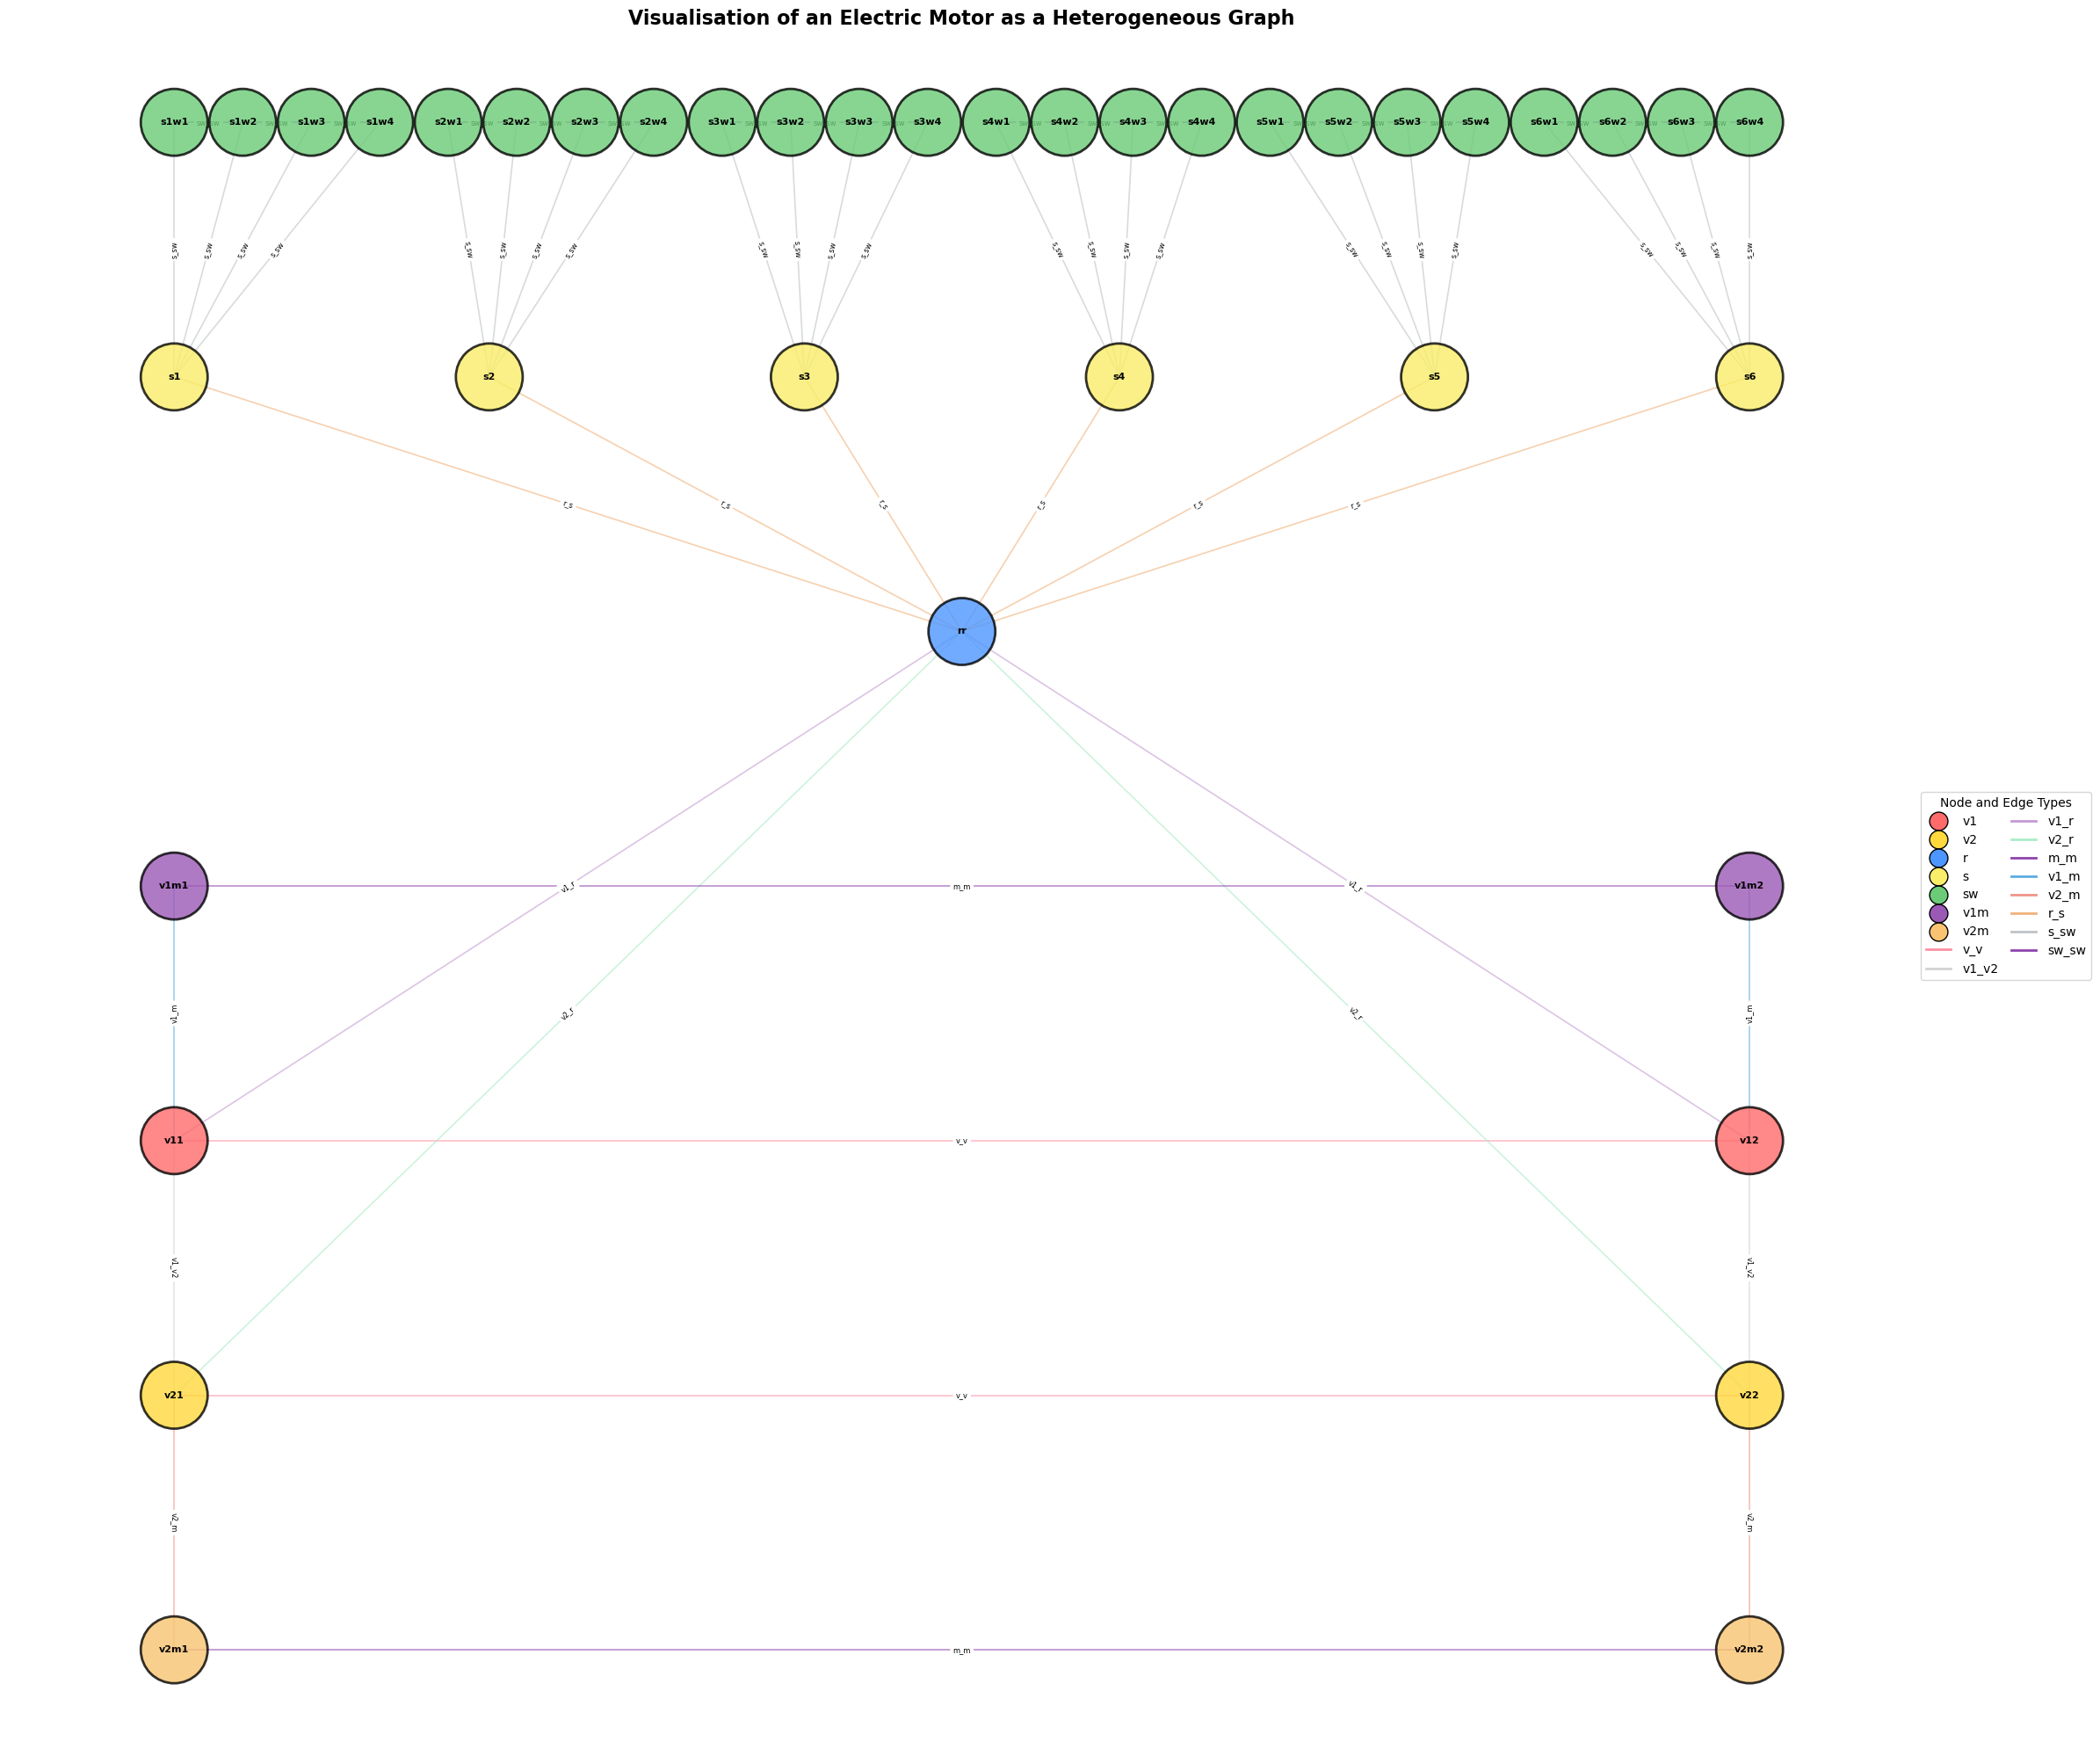
\includegraphics[width=0.9\textwidth]{./ReportImages/graph.png} 
    \caption{HetGraph}
    \label{fig:Graph}
\end{figure}

\newpage 

\chapter*{Modelling}
\addcontentsline{toc}{chapter}{Modelling}
Since we aim to predict continuous vector values, we model this task into a regression problem

We find the heterogeneous graph to be most apt for our use case with its different node and edge types. As it preserves both the structural and semantics of our data.
Heterogeneous graph Neural Networks generally work by having separate non linear functions convolve over each edge type during message computation and over each node type when aggregating the learned information.

\newpage 

\chapter*{Experiments and Results}
\addcontentsline{toc}{chapter}{Experiments and Results}
Firstly we train a MLP on the tabular representation of the data.
We have used MinMax Scaler for normalization of both the input and targets.
MSE loss function is used for the regression problem and Adam optimizer is used for optimization.
We have the first results on the 2D KPI-Mgrenz prediction.
These results are only considering about 400 examples. The dataset was split into training-validation(80:20) excluding test examples of about 19 examples.
\begin{figure}[h]
    \centering
    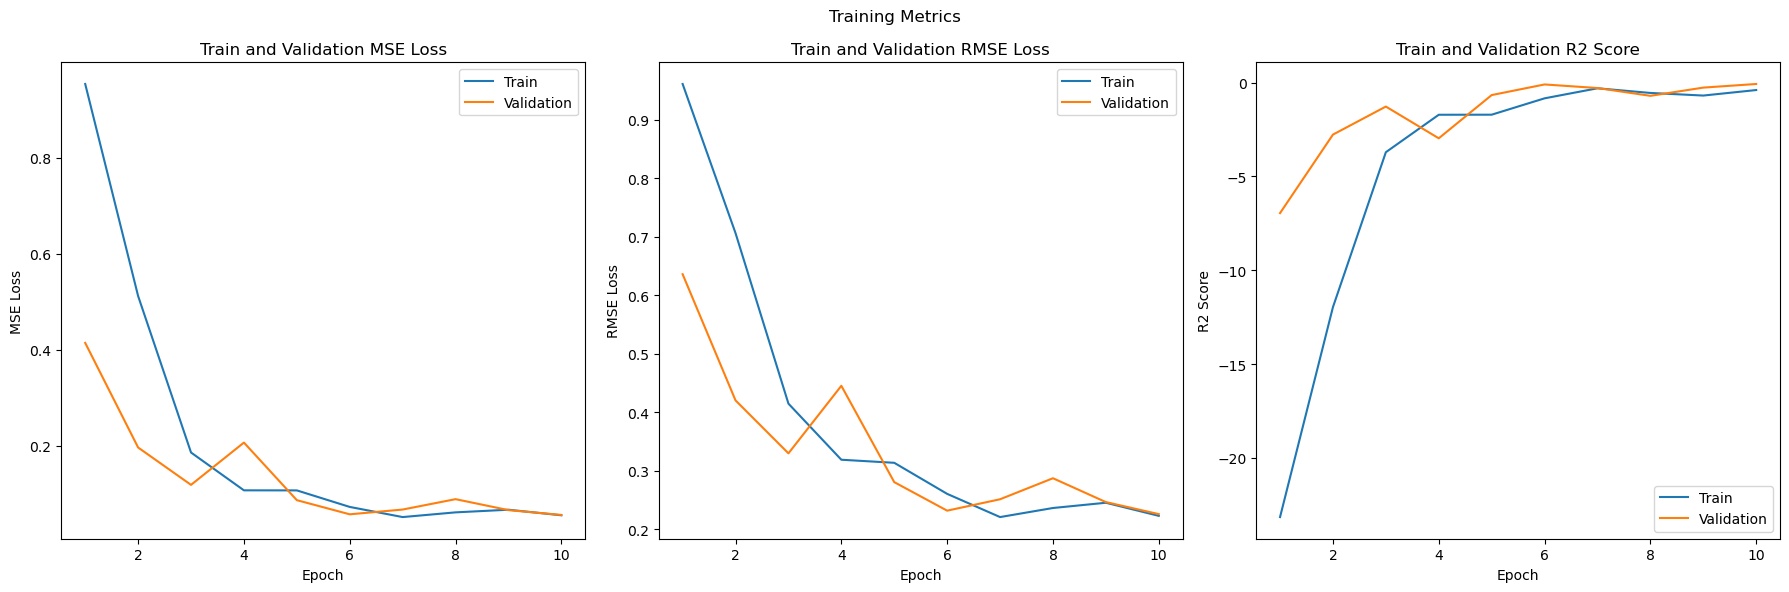
\includegraphics[width=0.95\textwidth]{./ReportImages/mlp_training_kpi2d.png} 
    \caption{MLP Training Plots for 2D KPI(Mgrenz)} 
    \label{fig:MLP Training Plots for 2D KPI(Mgrenz)}
\end{figure}

From the training plots we see that the model has converged after having run for 10 epochs with a learning rate of 0.0075.

The results of the MLP model from inference is as below:

\begin{figure}[h]
    \centering
    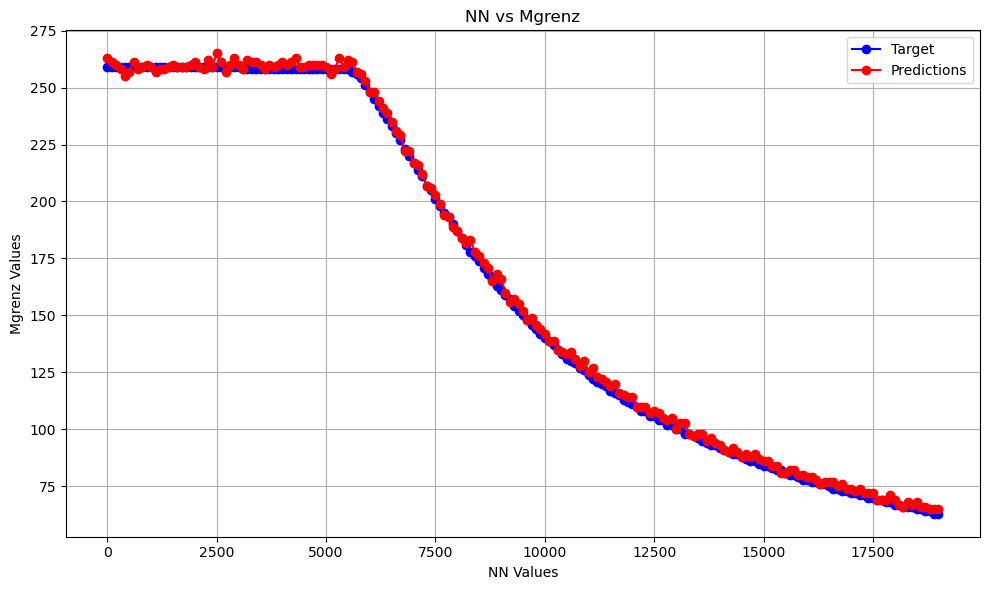
\includegraphics[width=0.75\textwidth]{./ReportImages/mlp_kpi2d_prediction.png} 
    \caption{MLP Training Results for 2D KPI(Mgrenz)} 
    \label{fig:MLP Training Results for 2D KPI(Mgrenz)}
\end{figure}

We see a good fit of the model to the data with R2 score approaching close to 1.
We have also enabled saving the trained model locally so it can be loaded on demand by the client to run inference.
\newpage 

\chapter*{Conclusion}

\newpage 

\newpage 

\listoffigures

\newpage 

\newpage 

\listoftables

\newpage 

\newpage 

\chapter*{Appendix}
\addcontentsline{toc}{chapter}{Appendix}

\newpage 

\newpage 

\chapter*{Bibliography}
\addcontentsline{toc}{chapter}{Bibliography}
\newpage 

\newpage 

\chapter*{Declaration on oath}
\addcontentsline{toc}{chapter}{Declaration on oath}

\vspace{1cm}

\noindent I hereby certify that I have written my master thesis independently and have not yet submitted it for examination purposes elsewhere. All sources and aids used are listed, literal and meaningful quotations have been marked as such.

\vspace{3cm}
\hfill\rule{15cm}{0.4pt} % Horizontal line for the signature aligned to the right

\begin{center}
    Lilly Abraham K64889, 11.12.2024 % Placeholder for the signature and date
\end{center}

\newpage 

\chapter*{Consent to Plagiarism Check}
\addcontentsline{toc}{chapter}{Consent to Plagiarism Check}
\vspace{1cm}

\noindent I hereby agree that my submitted work may be sent to PlagScan (www.plagscan.com) in digital form for the purpose of checking for plagiarism and that it may be temporarily (max. 5 years) stored in the database maintained by PlagScan as well as personal data which are part of this work may be stored there.

\vspace{0.5cm}

\noindent Consent is voluntary. Without this consent, the plagiarism check cannot be prevented by removing all personal data and protecting the copyright requirements. Consent to the storage and use of personal data may be revoked at any time by notifying the faculty.


\vspace{3cm}
\hfill\rule{15cm}{0.4pt} % Horizontal line for the signature aligned to the right

\begin{center}
    Lilly Abraham K64889, 11.12.2024 % Placeholder for the signature and date
\end{center}

\end{document}
